\documentclass[12pt]{article}
\usepackage[left=1cm, right=1cm, top=2cm,bottom=1.5cm]{geometry} 

\usepackage[parfill]{parskip}
\usepackage[utf8]{inputenc}
\usepackage[T2A]{fontenc}
\usepackage[russian]{babel}
\usepackage{enumitem}
\usepackage[normalem]{ulem}
\usepackage{amsfonts, amsmath, amsthm, amssymb, mathtools}
\usepackage{tabularx}
\usepackage{hhline}

\usepackage{accents}
\usepackage{fancyhdr}
\pagestyle{fancy}
\renewcommand{\headrulewidth}{1.5pt}
\renewcommand{\footrulewidth}{1pt}

\usepackage{graphicx}
\usepackage[figurename=Рис.]{caption}
\usepackage{subcaption}
\usepackage{float}

%%Наименование папки откуда забирать изображения
\graphicspath{ {./images/} }

%%Изменение формата для ввода доказательства
\renewcommand{\proofname}{$\square$  \nopunct}
\renewcommand\qedsymbol{$\blacksquare$}

%%Изменение отступа на таблицах
\addto\captionsrussian{%
	\renewcommand{\proofname}{$\square$ \nopunct}%
}
%% Римские цифры
\newcommand{\RN}[1]{%
	\textup{\uppercase\expandafter{\romannumeral#1}}%
}

%% Для удобства записи
\newcommand{\MR}{\mathbb{R}}
\newcommand{\MQ}{\mathbb{Q}}
\newcommand{\MN}{\mathbb{N}}
\newcommand{\MI}{\mathrm{I}}
\newcommand{\MJ}{\mathrm{J}}
\newcommand{\MH}{\mathrm{H}}
\newcommand{\MT}{\mathrm{T}}
\newcommand{\MU}{\mathcal{U}}
\newcommand{\MV}{\mathcal{V}}
\newcommand{\VN}{\varnothing}
\newcommand{\VE}{\varepsilon}

\theoremstyle{definition}
\newtheorem{defn}{Опр:}
\newtheorem{rem}{Rm:}
\newtheorem{prop}{Утв.}
\newtheorem{exrc}{Упр.}
\newtheorem{lemma}{Лемма}
\newtheorem{theorem}{Теорема}
\newtheorem{corollary}{Следствие}

\newenvironment{cusdefn}[1]
{\renewcommand\thedefn{#1}\defn}
{\enddefn}

\DeclareRobustCommand{\divby}{%
	\mathrel{\text{\vbox{\baselineskip.65ex\lineskiplimit0pt\hbox{.}\hbox{.}\hbox{.}}}}%
}
%Короткий минус
\DeclareMathSymbol{\SMN}{\mathbin}{AMSa}{"39}
%Длинная шапка
\newcommand{\overbar}[1]{\mkern 1.5mu\overline{\mkern-1.5mu#1\mkern-1.5mu}\mkern 1.5mu}
%Функция знака
\DeclareMathOperator{\sgn}{sgn}

%Обозначение константы
\DeclareMathOperator{\const}{\text{const}}

%Интеграл в большом формате
\DeclareMathOperator{\dint}{\displaystyle\int}

\newcommand{\smallerrel}[1]{\mathrel{\mathpalette\smallerrelaux{#1}}}
\newcommand{\smallerrelaux}[2]{\raisebox{.1ex}{\scalebox{.75}{$#1#2$}}}

\newcommand{\smallin}{\smallerrel{\in}}
\newcommand{\smallnotin}{\smallerrel{\notin}}

\newcommand*{\medcap}{\mathbin{\scalebox{1.25}{\ensuremath{\cap}}}}%
\newcommand*{\medcup}{\mathbin{\scalebox{1.25}{\ensuremath{\cup}}}}%

%Скалярное произведение
\DeclarePairedDelimiterX{\inner}[2]{\langle}{\rangle}{#1, #2}

%Подпись символов снизу
\newcommand{\ubar}[1]{\underaccent{\bar}{#1}}

\begin{document}
\lhead{Математический анализ - \RN{2}}
\chead{Шапошников С.В.}
\rhead{Лекция - 5}

\section*{Сходимость в нормированных пространствах}
$X$ - линейное (над $\MR$) пространство. На нем определена функция $\|\cdot\|\colon X \to [0, +\infty)$, удовлетворяющая свойствам:
\begin{enumerate}[label ={\arabic*)}]
	\item $\|x\| = 0 \Leftrightarrow x = 0$;
	\item $\|\alpha x \| = |\alpha|{\cdot}\|x\|$;
	\item $\|x + y\| \leq \|x\| + \|y\|$;
\end{enumerate}

Полезное неравенство: $\big| \|x\| - \|y\| \big| \leq \|x - y\|$.

\begin{defn}
	На нормированном пространстве $x_n \to x \Leftrightarrow \|x_n - x\| \to 0$.
\end{defn}

\subsection*{Нормы в $\MR^n$}
С точки зрения сходимости последовательностей, все нормы в $\MR^n$ эквивалентны.
\begin{theorem}
	Если $\|\cdot\|_1$ и $\|\cdot\|_2$ - произвольные нормы на $\MR^n$, то $\exists$ числа $c_1, c_2 > 0$:
	$$
	c_1 \|x\|_1 \leq \|x\|_2 \leq c_2 \|x\|_1, \, \forall x \in \MR^n
	$$
\end{theorem}
\begin{proof}
	Достаточно доказать для случая, когда $\|x\|_2 = \sqrt{x_1^2 + \dotsc + x_n^2}$, поскольку, если можем доказать, что $\|x\|_1 \leq c_2 \|x\|_2 \wedge \|x\|_1 \geq c_1 \|x\|_2$, то можем оценить любые две нормы:
	$$
		\|x\|_1 \leq c_2\|x\|_2 \leq c_2{\cdot}c_3\|x\|_3 \wedge \|x\|_1 \geq c_1 \|x\|_2 \geq c_1{\cdot}c_4\|x\|_3
	$$
	Напомним, что в $\MR^n$ есть базис $e_k = (0,\dotsc,0,\underset{k}{1},0, \dotsc, 0)$ и $x = x_1 e_1 + \dotsc + x_n e_n$. Возьмем первую норму $\|x\|_1 = \|x_1 e_1 + \dotsc + x_n e_n \|_1$, тогда:
	$$
		\|x_1 e_1 + \dotsc + x_n e_n \|_1 \leq \|x_1 e_1\|_1 + \dotsc + \|x_n e_n\|_1 = |x_1|{\cdot}\|e_1\|_1 + \dotsc + |x_n|{\cdot}\|e_n\|_1 \leq \|x\|_2(\|e_1\|_1 + \dotsc + \|e_n\|_1)
	$$
	где последнее неравенство верно в силу леммы. И таким образом:
	$$
		\|x\|_1 \leq \|x\|_2(\|e_1\|_1 + \dotsc + \|e_n\|_1) = \|x\|_2 c_1
	$$
	Таким образом, используя $0 \leq \|x_n -x \|_1 \leq c_2 \|x_n - x\|_2 \to 0$ получим:
	$$
		\|x\|_1 \leq c_1 \|x\|_2 \wedge x_n \xrightarrow[]{\|\cdot\|_2}x \Rightarrow x_n \xrightarrow[]{\|\cdot\|_1}x
	$$
	то есть сходимость по Евклидовой норме дает сходимость по норме $1$.
	
	Предположим, что $\nexists \, C > 0 \colon \|x\|_2 \leq C \|x\|_1 \Rightarrow \forall N \in \MN, \exists \, x_N \neq 0 \colon \|x_N\|_2 > N{\cdot}\|x_N\|_1$. От умножения на положительный скаляр, неравенство не изменится $\Rightarrow$ возьмем $y_N = \tfrac{x_N}{\|x_N\|_2} \Rightarrow \|y_N\|_2 > N{\cdot}\|y_N\|_1$, тогда последовательность $y_N$ обладает следующими свойствами:
	\begin{enumerate}[label ={\arabic*)}]
		\item $\|y_N\|_2 = 1$;
		\item $\dfrac{1}{N} = \dfrac{\|y_N\|_2}{N} > \|y_N\|_1 \Rightarrow \|y_N\|_1 \xrightarrow[]{N \to \infty} 0$;
	\end{enumerate} 
	Поскольку $\|y_N\|_2 = 1 \Rightarrow$ эта последовательность ограничена $\Rightarrow$ по теореме Больцано $\exists \, y_{N_k} \xrightarrow[]{\|\cdot\|_2} y$, тогда $\|y_{N_k}\|_2 = 1 \to \|y\|_2 = 1$. Но если есть сходимость по Евклидовой норме $\|\cdot\|_2$, то обязательно $y_{N_k} \xrightarrow[]{\|\cdot\|_1} y$, но $y_{N_k} \xrightarrow[]{\|\cdot\|_1} 0$ и $y = 0 \Rightarrow y = 0\wedge \|y\|_2 = 1 \Rightarrow$ противоречие.  
\end{proof}
Таким образом, на $\MR^n$ все нормы эквивалентнты $\Rightarrow$ с точки зрения сходимости, все что верно для Евклидовой нормы, будет верно и для других норм, например, что $\MR^n$ - полное пространство.

\begin{defn}
	Если нормированное пространство полно, то его называют \uwave{Банаховым} пространством. 
\end{defn}

\subsection*{Ряды в нормированных пространствах}
В линейных нормированных пространствах можем складывать $\Rightarrow$ можем сказать, что такое сумма ряда: 
$$\displaystyle \sum\limits_{n = 1}^{\infty} x_n = \lim\limits_{N \to \infty} \displaystyle \sum\limits_{n = 1}^{N} x_n =  \lim\limits_{N \to \infty} S_N$$
Если ряд сходится, то $x_n = \displaystyle \sum\limits_{k = 1}^{n} x_k - \sum\limits_{k = 1}^{n-1}x_k \to 0$ (необходимое условие выполнено).

\begin{prop}
	Если нормированное пространство полно, то если $\displaystyle\sum\limits_{n = 1}^{\infty} \|x_n\|$ - сходится $\Rightarrow \displaystyle\sum\limits_{n = 1}^{\infty} x_n$ - сходится.
\end{prop}
\begin{proof}
	Пространство полно $\Rightarrow$ будем проверять критерий Коши, пусть $M < N$:
	$$
		\Bigg\| \sum\limits_{n = 1}^{N} x_n - \sum\limits_{n = 1}^{M}x_n\Bigg\| = \Bigg\|\sum\limits_{n = M+1}^{N} x_n\Bigg\| \leq \sum\limits_{n = M+1}^{N} \|x_n\| \xrightarrow[]{N,M \to \infty} 0
	$$
	по критерию Коши для числового ряда. Таким образом, последовательность частичных сумм - фундаментальна $\Rightarrow$ эта последовательность сходится.
\end{proof}

\subsection*{Матрицы в нормированных пространствах}
Линейное пространство матриц размера $n\times n,\, M_n$ (элементы из $\MR$). С точки зрения пространств этот объект это $\MR^{n^2} = M_n$. Зададим норму следующим образом: 
$$
\|A\| = \sup\limits_{x \neq 0}\dfrac{\|Ax\|}{\|x\|}, \, \text{где } \|x\| = \|x\|_2 = \sqrt{x_1^2 + \dotsc + x_n^2}
$$
\textbf{\uline{Случай}} $n=1$: $\|a\| = \sup\limits_{x\neq 0}\dfrac{|ax|}{|x|} = |a|$. $x \mapsto ax$ - растяжение, $a$ - это коэффициент гомотетии. 

\textbf{\uline{Случай}} $n=2$: $A = \begin{pmatrix} a & 0\\ 0 & b \end{pmatrix} \Rightarrow x^T = (x_1,x_2) \Rightarrow Ax = \begin{pmatrix} a & 0\\ 0 & b \end{pmatrix} \begin{pmatrix} x_1 \\x_2 \end{pmatrix} = \begin{pmatrix} a x_1 \\ b x_2 \end{pmatrix} \Rightarrow \|Ax\| = \sqrt{a^2 x_1^2 + b^2 x_2^2}$, таким образом получим:
$$
	\dfrac{\|Ax\|}{\|x\|} = \dfrac{\sqrt{a^2 x_1^2 + b^2 x_2^2}}{\|x\|} = \sqrt{a^2 \dfrac{x_1^2}{\|x\|^2} + b^2\dfrac{x_2^2}{\|x\|^2}} = \Big\|A\tfrac{x}{\|x\|}\Big\|, \,\text{где } \dfrac{x_1^2}{\|x\|^2} + \dfrac{x_2^2}{\|x\|^2} = \dfrac{x_1^2 + x_2^2}{x_1^2 + x_2^2} = 1 \Rightarrow y_i^2 = \dfrac{x_i^2}{\|x\|^2}
$$
Сделав замену хотим $a^2y_1^2 + b^2 y_2^2 \to \max$ при условии, что $y_1^2 + y_2^2 = 1$. 

Пусть $b^2 \geq a^2$. Выразим $y_1^2$: 
$$y_1^2 = 1- y_2^2 \Rightarrow a^2(1- y_2^2) + b^2 y_2^2 = a^2 + (b^2 - a^2)y_2^2, \, y_2 \in [0,1]$$ 
Тогда $\Rightarrow y_2^2 = 1 \Rightarrow  a^2 + (b^2 - a^2)y_2^2 = b^2$. Таким образом, получим $\|A\| = \max\{|a|, |b| \}$. 

Что делает это преобразование? Геометрически, оно в $a$ раз вытягивает $x_1$ и в $b$ раз вытягивает $x_2$. Получилось, что норма равна максимальному коэффициенту растяжения. 

\uline{Смысл нормы}: измеряет во сколько раз максимально вытягиваются вектора. 

Очевидно, что $\|A\|$ - это конечное число, поскольку вычисления производятся на единичных векторах с использованием матрицы с фиксированными числами.

Пусть $x_1^2 + x_2^2 = 1$, рассмотрим общий случай:
$$
	\begin{pmatrix} a & b\\ c & d \end{pmatrix}\begin{pmatrix} x_1 \\x_2 \end{pmatrix} = \begin{pmatrix} ax_1 + bx_2 \\ c x_1 + d x_2 \end{pmatrix} \Rightarrow ax_1 + bx_2 \leq |a| + |b| \wedge cx_1 + dx_2 \leq |c| + |d|
$$
Координаты вектора ограничены конкретными числами $\Rightarrow$ ограниченный вектор $\Rightarrow$ длина этого вектора также ограничена \Big($\leq \sqrt{(|a| + |b|)^2 + (|c| + |d|)^2}$\Big) $\Rightarrow \dfrac{\|Ax\|}{\|x\|}$ - ограничено $\Rightarrow$ разумно брать точную верехнюю грань. Точная верхняя грань $\sup\limits_{x \neq 0} \dfrac{\|Ax\|}{\|x\|}$ - это наименьшее из чисел $C \colon \|Ax\| \leq C \|x\| \Rightarrow$ нормой $A$ мы смотрим самую точную границу этого растяжения: в какое наименьшее число раз вектор может удлиниться.

Остается вопрос: почему это норма?

\begin{prop}
	Пусть 
	$$
	\|A\| = \sup\limits_{x \neq 0}\dfrac{\|Ax\|}{\|x\|}, \, \text{где } \|x\| = \|x\|_2 = \sqrt{x_1^2 + \dotsc + x_n^2}
	$$
	тогда справедливо следующее:
	\begin{enumerate}[label ={(\arabic*)}]
		\item $\|A\|$ - норма;
		\item $\|A{\cdot}B\| \leq \|A\|{\cdot}\|B\|$;
	\end{enumerate}
\end{prop}
\begin{proof}\hfill
	\begin{enumerate}[label ={\arabic*)}]
		\item Рассмотрим свойства нормы:
		\begin{enumerate}[label ={(\arabic*)}]
			\item $\|A\| \geq 0$ - очевидно, $\|A\| = 0 \Rightarrow \forall x, \, Ax = 0 \Leftrightarrow A = 0$ (подставляем базисные вектора, получаем нулевые столбцы);
			\item $\|\alpha A\| = \sup\limits_{x \neq 0} \dfrac{\|\alpha Ax\|}{\|x\|} = \sup\limits_{x \neq 0} \dfrac{|\alpha|\| Ax\|}{\|x\|} = |\alpha| \sup\limits_{x \neq 0} \dfrac{\| Ax\|}{\|x\|} = |\alpha|\|A\|$;
			\item $\dfrac{\|(A+B)x\|}{\|x\|} = \dfrac{\|Ax + Bx\|}{\|x\|} \leq \dfrac{\|Ax \|}{\|x\|}  + \dfrac{\|Bx\|}{\|x\|} \leq \|A\| + \|B\| \Rightarrow \sup\limits_{x \neq 0}\dfrac{\|(A+B)x\|}{\|x\|} \leq \|A\| + \|B\| \Rightarrow$\\ $\Rightarrow \|A+B\| = \sup\limits_{x \neq 0}\dfrac{\|(A+B)x\|}{\|x\|} \leq \|A\| + \|B\|$;
		\end{enumerate} 
		\item Заметим, что $\forall x, \, \|Ax\| \leq \|A\|{\cdot}\|x\|$, так как $\dfrac{\|Ax\|}{\|x\|} \leq \|A\|$. Тогда
		$$
		\dfrac{\|(A{\cdot}B)x\|}{\|x\|} = \dfrac{\|A(Bx)\|}{\|x\|} \leq \|A\|{\cdot}\dfrac{\|Bx\|}{\|x\|} \leq \|A\|{\cdot}\|B\|{\cdot}\dfrac{\|x\|}{\|x\|} = \|A\|{\cdot}\|B\| \Rightarrow
		$$ 
		$$
		\Rightarrow \sup\limits_{x\neq 0}\dfrac{\|(A{\cdot}B)x\|}{\|x\|} = \|A{\cdot}B\| \leq \|A\|{\cdot}\|B\|
		$$
	\end{enumerate}
\end{proof}
\begin{rem}
	В общем случае, равенство не будет достигнуто.
\end{rem}
\begin{exrc}\hfill
	\begin{enumerate}[label ={\arabic*)}]
		\item Привести пример, когда $\|AB\| < \|A\|{\cdot}\|B\|$;
		\item Попробовать найти норму $\begin{pmatrix} a & b\\ c & d \end{pmatrix}$;
	\end{enumerate}
\end{exrc}

Пространство $(M_n, \|\cdot\|)$ - нормированное и зная, что $M_n = \MR^{n^2} \Rightarrow $ все нормы эквивалентны  $\Rightarrow$ относительно всех норм это полное пространство $\Rightarrow (M_n, \|\cdot\|)$ - банахово пространство.

\begin{defn}
	$e^A = \MI + A + \dfrac{A^2}{2!} + \dotsc + \dfrac{A^n}{n!} + \dotsc $ .
\end{defn}
\begin{rem}
	Чтобы это стало корректным определением, надо понять, почему этот ряд сходится.
\end{rem}
В полном пространстве, для сходимости достаточно проверить, что сходится ряд из норм: $\displaystyle \sum\limits_{n = 0}^{\infty} \bigg\|\dfrac{A^n}{n!}\bigg\|$:
$$
	\sum\limits_{n = 0}^{\infty} \bigg\|\dfrac{A^n}{n!}\bigg\| \leq \sum\limits_{n = 0}^{\infty} \dfrac{1}{n!}\|A\|^n = e^{\|A\|}
$$
Таким образом, ряд $\displaystyle \sum\limits_{n = 0}^{\infty} \bigg\|\dfrac{A^n}{n!}\bigg\|$ - сходится $\Rightarrow e^A = \displaystyle \sum\limits_{n = 0}^{\infty} \dfrac{A^n}{n!}$ - сходится.

\begin{rem}
	Верно ли, что $e^{A + B} = e^A{\cdot}e^B$? Ответ: нет.
	
\end{rem}

\begin{exrc}
	Если $[A,B] = AB - BA = 0$, то $e^{A + B} = e^A{\cdot}e^B$. Верно ли будет обратное? (да, но при дополнительном условии).
\end{exrc}

\begin{exrc}
	Найти $e^A$, где $\underset{n \times n}{A} = \begin{pmatrix} 0 & 1 & 0 & \dotsc & 0 \\ 0 & 0 & 1 & \dotsc & 0 \\ \vdots & \vdots & \vdots & \ddots & \vdots \\ 0&0&0&\dotsc&1\\
	0& 0& 0&\dotsc &0  \end{pmatrix}$.
\end{exrc}

\newpage
\section*{Пространство ограниченных функций}
Пусть $X \neq \VN$. Обозначаем \uwave{пространство ограниченных функций}:
$$
	B(X) = \{\, f\colon X \to \MR \mid \sup\limits_{x \in X}|f(x)| < \infty\,\}
$$
это линейное пространство и на нем есть метрика, зададим её сразу нормой:
$$
	\|f\| = \sup\limits_{x \in X}|f(x)|
$$
\begin{exrc}
	Проверить, что $\|f\|$ это действительно норма.
\end{exrc}
$(B(x),\|\cdot\|)$ - нормированное пространство, рассмотрим сходимость на этом пространстве:
$$
	f_n \to f \Leftrightarrow \|f_n - f\| \to 0 \Leftrightarrow \sup\limits_{x \in X}|f_n(x) - f(x)| \to 0
$$
то есть: 
$$
	\forall \VE > 0, \exists \, N \colon \forall n > N, \, \sup\limits_{x \in X}|f_n(x) - f(x)| < \VE
$$
это \uwave{равномерная сходимость}.

\textbf{Пример}: $f_n(x) = \dfrac{x}{n}, \, X = [0,1]$.
\begin{figure}[H]
	\centering
	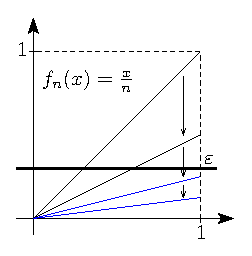
\includegraphics[width=0.25\textwidth]{5_1.eps}
	\caption{Пример функции с равномерной сходимостью.}
	\label{5_1}
\end{figure}
Все функции равномерно приближаются к нулю: для всякого уровня $\VE$ можно указать номер, когда все функции целиком лежат ниже этого уровня $\VE$. В этом случае, если мы возьмем супремум: 
$$\sup\limits_{x \in X}|f_n| = \dfrac{1}{n} \to 0$$

\textbf{Пример}: $f_n(x) = x^n, \, X = (0,1)$. В этом случае, указать единый номер, когда все функции ниже уровня $\VE$ не получится, поскольку функции сколь угодно близко к $1$ стремятся к значению выше изначально заданного $\VE$. Таким образом, есть поточечная сходимость, но нет равномерной сходимости.
\begin{figure}[H]
	\centering
	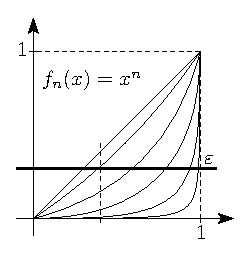
\includegraphics[width=0.25\textwidth]{5_2.eps}
	\caption{Пример функции без равномерной сходимости.}
	\label{5_2}
\end{figure}
Действительно, рассмотрим супремум: 
$$\sup\limits_{x \in X}|f_n| = 1 \nrightarrow 0$$ 
хотя в каждой отдельно взятой точке есть стремление к $0$.

Можно ли придумать метрику, которая задавала бы поточечную сходимость?

\begin{prop}
	На $B([0,1])$ не существует метрики $\rho \colon \rho(f_n, f) \to 0 \Leftrightarrow f_n(x) \to f(x), \, \forall x$ (поточечная сходимость).
\end{prop}
\begin{proof}
	(От противного): предположим, что такая $\rho$ существует. Рассмотрим шар $B(0,r)$ по этой метрике. Возьмем последовательность отрезков: каждый следующий меньше предыдущего, их бесконечное число, стремящихся к точке $1$, но не доходящих до неё.
	\begin{figure}[H]
		\centering
		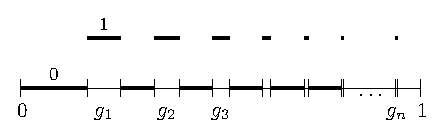
\includegraphics[width=0.55\textwidth]{5_3.eps}
		\caption{Доказательство несуществования метрики с поточечной сходимостью.}
		\label{5_3}
	\end{figure}
	Возьмем последовательность функций $\{g_n\}$, такую что на этих отрезках она принимает значения $1$, вне этих отрезков значения $0$. Понятно, что $g_n(x) \to 0, \, \forall x  \in [0,1]$ (поточечно), тогда 
	$$
		\exists \, n \colon g_n \in B(0,r) = \{g\mid \rho(0,g) < r\}
	$$
	Таким образом, для любого шара мы научились находить такой отрезок, что функция равна $1$ на этом отрезке и $0$ вне него, лежит в этом шаре.
	
	Возьмем отрезок $[0,1]$, на нем возьмем шар $B(0,1)$, найдем отрезок и функцию $f_1$ на нем, такую что она лежит в этом шаре. Затем возьмем шар $B(0,\frac{1}{2})$ и внутри предыдущего отрезка, аналогичным построением последовательности функций, найдем другой отрезок и функцию $f_2$ на нем, которая лежит в шаре $B(0,\frac{1}{2})$. 
	
	Продолжим построение, получим последовательность вложенных отрезков и последовательность функций $\{f_n\}$, которые лежат в этих шарах: $f_n \in B(0,\frac{1}{n})$. У вложенной системы отрезков есть общая точка $c \colon f_n(c) = 1, \, \forall n$. С другой стороны $\forall n, \, f_n \in B(0,\frac{1}{n}) \Rightarrow \rho(f_n, 0) < \frac{1}{n} \Rightarrow f_n \to 0$, но $f_n(c) = 1 \Rightarrow$ противоречие.
\end{proof}

\end{document}